\section{The web application}
\label{sec:website}

This section describes the main characteristics of the website, and the technologies it is built with.

\subsection{Single-page application}
\label{ssec:spa}

\url{https://www.konnektid.com/} is built as a single-page application (\guillemotleft{} SPA \guillemotright{}).
A SPA distinguishes from other web applications by loading one unique web page, and the totality of its necessary code, right from the start.
After that initial load, all of the logic (presentation, business, routing\ldots) is handled by the client side, in Konnektid's case through JavaScript.
And when the user interacts with the page, only the affected parts of the user interface (\guillemotleft{} UI \guillemotright{}) are updated.

This is achieved by using a specific architecture introduced on {\sc figure}~\ref{fig:spaArchi}, in which the data (\guillemotleft{} Model
\guillemotright{} layer) is separated from its presentation (\guillemotleft{} View \guillemotright{} layer)\cite{spa}.

\begin{figure}[H]
    \centering
    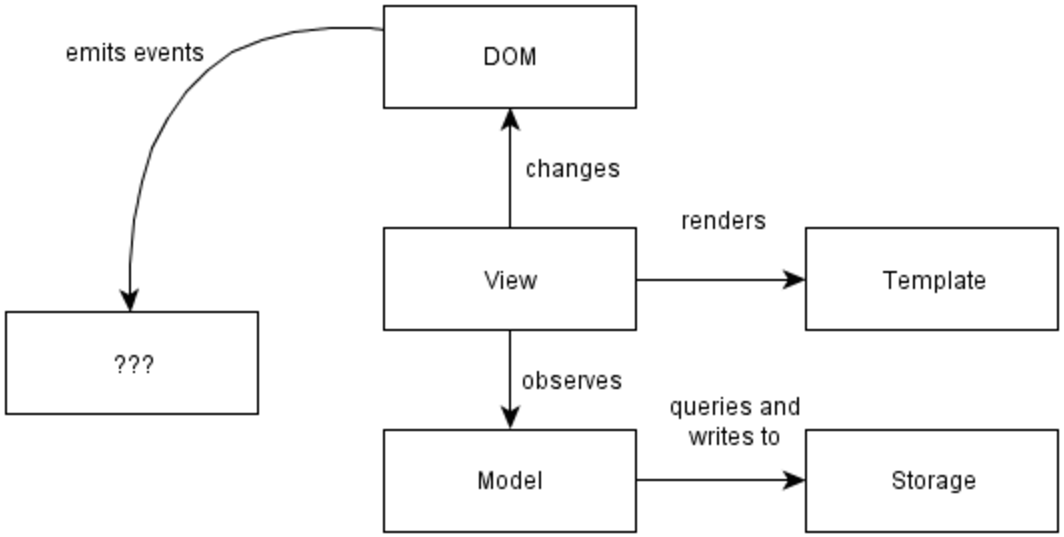
\includegraphics[scale=0.5]{figure/spaArchi.png}
    \caption{The usual structure of a single-page application.}
    \label{fig:spaArchi}
\end{figure}

A few more details about the different parts of the architecture:
\begin{itemize}[noitemsep]
    \item DOM~\footnote{Document Object Model: provides a representation of the document structured as a tree, and methods to access it.} is write-only:
    no data is read from it, it just outputs HTML, operations and events;
    \item Models handles all the data and state of the application;
    \item Views update the UI, depending on DOM events and models, as pictured on {\sc figure}~\ref{fig:view}.
\end{itemize}

\begin{figure}[H]
    \centering
    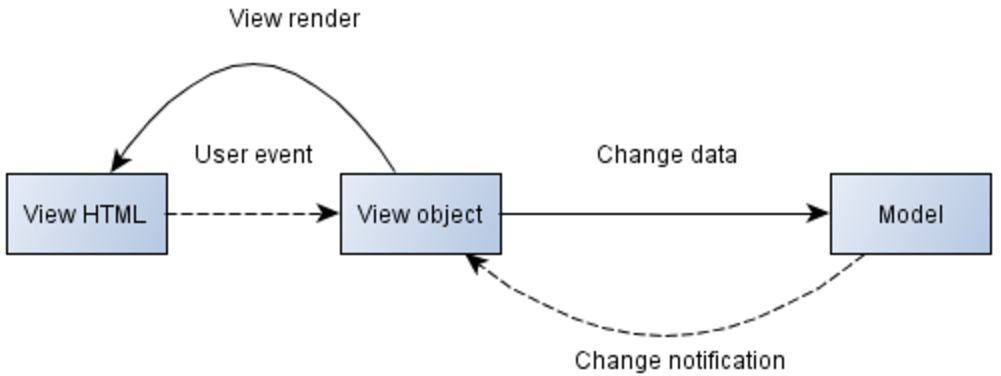
\includegraphics[scale=0.6]{figure/view.png}
    \caption{Possible interactions between the View and the other layers.}
    \label{fig:view}
\end{figure}

SPAs support communication between multiple components, each of them having intermediate states (menu open, item selected, etc), which is difficult to
implement with other approaches such as server-side rendering. However, this affects the run-time state of the application (i.e. what the application looks like when it is
running in a browser), as the whole state cannot fit inside one URL. For SPAs, the level of details in URLs is reduced, usually by focusing on the primary activity
of the page and skipping the secondary activities (for instance modals) that will be reset to default state in case of reload.

By avoiding page reloads, SPAS bring a more responsive and fluid user experience and a better overall performance.
There are various techniques and frameworks available for implementing SPAs.
Among them, Konnektid uses several that are described in {\sc subsection}~\ref{ssec:frameworks}.

\subsection{Frameworks and libraries}
\label{ssec:frameworks}

The website is principally developed in JavaScript, HTML and SCSS. It features a certain number of frameworks and librairies: the main ones are described in the present section.

\subsubsection{ReactJS}
\label{sssec:react}

ReactJS is an open source frontend JavaScript library, used to create reusable components that can be composed in order to build user interfaces. It differs from other libraries by its automatic way of keeping the DOM up-to-date. ReactJs implements a \guillemotleft{} virtual DOM \guillemotright{}, i.e. a lightweight representation of the view, from which the markup is created and inserted into the actual DOM. Then for each component, at initialization a \textit{render()} method is called, that generates the corresponding slice of DOM. Then, whenever the data changes or events are emitted, \textit{render()} returns a minimal set of modifications to apply to the DOM.
This makes web applications much faster, and easier to build~\cite{whyReact}.

ReactJS components act just like functions: they take data as input and output the corresponding UI in return. They can manipulate two different kinds of data:

\textbf{The state} It is a set of internal data, that can only be updated by the component itself using the \textit{setState()}  method. All React components do not necessary have state: if they do, they are called \guillemotleft{} stateful \guillemotright{} (or \guillemotleft{} smart \guillemotright{}), in opposition to \guillemotleft{} stateless \guillemotright{} (or \guillemotleft{} dumb \guillemotright{}) for the others. Stateful components access their state via \textit{this.state}.

\textbf{The props} These properties are passed down to the component by its parents, and can be accessed by calling \textit{this.props}. They cannot be modified by the component, but to avoid issues if not provided it is possible to define default values.

So ReactJS can be summarized as: \framebox{\textbf{component(props, state) => UI}}

A good practice it to keep the number of stateful components as low as possible~\cite{state}. Konnektid follows this advice, 
by implementing most of its components presentational. When a state is really needed, a \guillemotleft{} container \guillemotright{} is created on top in order to handle the logic. This parent can then pass properties down to the stateless component which only handles the rendering. This technique respects another recommanded convention: the single responsibility principle (each class or module should only have one task to handle). 

Most developers (including the ones at Konnetid) use React with JSX, a preprocessor step that adds XML-like syntax to JavaScript.
It makes the code easier to debug, and faster thanks to the optimization performed during compilation~\cite{whyJsx}. {\sc figure}~\ref{fig:jsx} shows that code written in JSX is much more readable than raw JavaScript.

\begin{figure}[H]
    \centering
    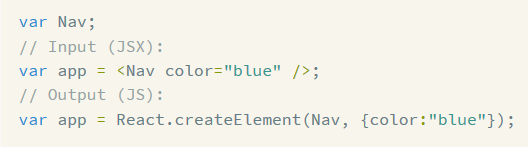
\includegraphics[scale=0.9]{figure/jsx.png}
    \caption{An example of JSX code and its JavaScript output.}
    \label{fig:jsx}
\end{figure}

\subsubsection{Redux}
\label{sssec:redux}

Redux is a predictable container for JavaScript applications~\cite{reduxDoc}, in other words, it handles the logic and the data so that React components only have to deal with the presentation. It stocks the whole state of the application into one object tree called \guillemotleft{} store \guillemotright{}. 

The store provides methods to access the state (\textit{store.getState()}) and to modify it (\textit{store.dispatch()}). The second method takes a parameter, an \guillemotleft{} action \guillemotright{}, which is a JavaScript object describing what happened and containing at least a type (usually a constant). Actions are produced by specific functions called \guillemotleft{} action creators \guillemotright{}, as shown on {\sc figure}~\ref{fig:action}.

\begin{figure}[H]
    \centering
    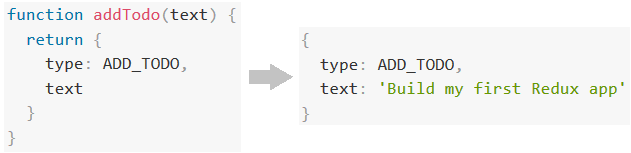
\includegraphics[scale=0.9]{figure/action.png}
    \caption{An example of action creator and one of its possible outputs.}
    \label{fig:action}
\end{figure}

To specify how the application's state is transformed by actions, Redux uses \guillemotleft{} reducers \guillemotright{}. They are pure functions~\footnote{Functions that always return the same result given the same argument(s), because they have no internal state.} with no side effects, that take the previous state and an action, and output an object containing the new state. The previous state is never modified, so that it can be returned in default case (e.g. for an unknown action). The Redux behaviour is illustrated on {\sc figure}~\ref{fig:reduxSumup}.

\begin{figure}[H]
    \centering
    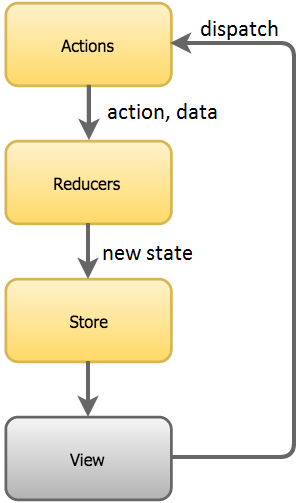
\includegraphics[scale=0.7]{figure/reduxFlow.png}
    \caption{A simplified diagram of how Redux works.}
    \label{fig:reduxSumup}
\end{figure}

To summarize, Redux works as follows: \framebox{\textbf{reducer(previousState, action) => newState}}.

\subsubsection{Node.js}
\label{sssec:node}

Konnektid's server-side code is mostly based on Node.js, an asynchronous event-driven JavaScript runtime. It is particularly efficient because it uses Google Chrome's open source V8 engine, that is able to quickly analyze and execute JavaScript code~\cite{v8}.

Node.js's non-blocking code architecture is one of the reasons why it is particularly fast: the program does not need to wait to finish an action before launching a new one~\cite{node}. This is achieved by associating each input/output operation (such as a database query) to a callback function that will be fired as soon as the operation is over. In between, the system can work on other tasks, as illustrated on {\sc figure}~\ref{fig:callback}.

\begin{figure}[H]
    \centering
    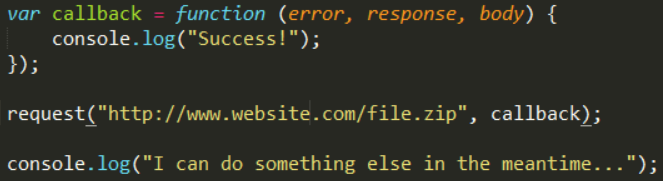
\includegraphics[scale=0.8]{figure/callback.png}
    \caption{An example of non-blocking code with a callback function.}
    \label{fig:callback}
\end{figure}

These non-blocking operations are possible in Node.js because they are handled by the multi-threaded system kernel, via an event loop~\cite{eventLoop}.

Finally, another strong suit of Node.js is its package ecosystem, npm, which allows developers to share solutions to particular issues~\cite{npm}. Anyone can reuse these pieces of code in their own projects, then npm facilitates checking on updates that were made and downloading them.

\subsubsection{GraphQL}
\label{sssec:grqphql}

GraphQL is used by Konnektid to communicate between the client and the server. To be understood by GraphQL, the queries must respect a specific format illustrated on the left side of {\sc figure}~\ref{fig:query}. They are then interpreted by the server and provide a result: an object containing all the required fields, similar to the right side of {\sc figure}~\ref{fig:query}.

\begin{figure}[H]
    \centering
    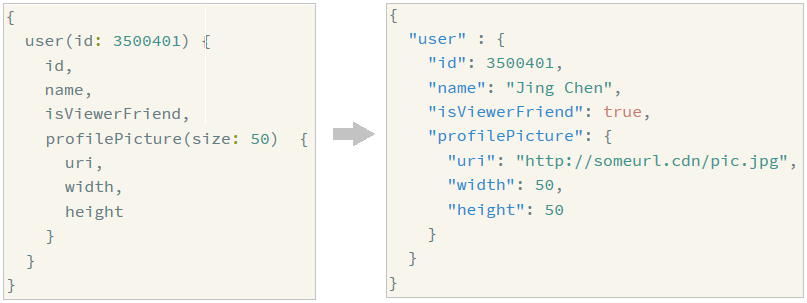
\includegraphics[scale=0.8]{figure/query.png}
    \caption{An example of GraphQL query and its result.}
    \label{fig:query}
\end{figure}

There are a few advantages to use GraphQL instead of REST APIs~\cite{graphQL}. First of all, as noticeable on {\sc figure}~\ref{fig:query}, the query is shaped just like the data it returns: as a hierarchy of fields. This makes it more natural to write and also easier to understand. Another particularity of GraphQL is that its queries are encoded in the client and not in the server, allowing to return exactly what the client asks for and nothing more. Moreover, GraphQL is strongly-typed: it controls both the correctness and the validity of the syntax of each query before executing it.

In the current section the main technologies have been introduced, now {\sc section}~\ref{sec:github} describes the development process and the use of Github inside the Konnekid team.
